\documentclass{./llncs2e/llncs}
\usepackage{graphicx}
\usepackage{fixltx2e}
\usepackage{mathtools}
\usepackage[nolist,nohyperlinks]{acronym}
% Maintain images and tables within their respective sections
\usepackage[section]{placeins}

% Scientific notation
\usepackage[scientific-notation=true, round-precision=2, round-mode=figures]{siunitx}

% For tables
\usepackage{multirow}

%For symbols like trademark
\usepackage{textcomp}

% To improve captions of tables
\usepackage{caption}
\captionsetup[table]{skip=10pt}

\pagestyle{plain}

%
% Change the margins
%
% \usepackage[margin=2.9cm]{geometry}

\begin{document}

% -------------------------------------
% Title
% -------------------------------------
\title{Check Please!}

\subtitle{Using Bluetooth beacons to enable a Smart Restaurant experience}
\author{Samuel Coelho, Miguel Pardal}
\institute{Instituto Superior T\'{e}cnico, Universidade de Lisboa
  \\
  \email{\{samuel.coelho, miguel.pardal\}@tecnico.ulisboa.pt}
}


\maketitle

% -------------------------------------
% Abstract and keywords
% -------------------------------------

%!TEX root = ../article.tex

% Abstract
\begin{abstract}
Proximity-based applications engage users while they are in the proximity of points of interest. These apps are becoming popular among the users of mobile devices.
Proximity based apps are triggered when the user is at specific geographic coordinates, but more interestingly, they can be triggered by tagged objects.
We introduce the concept of Smart Place which is a physical place where tags are placed in order to provide a service. Users with a mobile device capable of detecting such tags can use the provided service when they are in proximity of these tags.
Several technologies can be used to create tags.

In this dissertation, we analyze several location technologies in order to choose one that best fits the concept of Smart Place.
We have created a solution to develop proximity-based applications, based on this concept.
Also, two examples of Smart Places were built: the Smart Restaurant and Smart Museum.
The Smart Places apps allows anyone with a mobile device capable of detecting tags, to have access to any proximity-based service, based on our concept of Smart Place and created using the tool we developed.
This app was evaluated in terms of energy consumption and the results show that the battery drain can be acceptable making it a viable technical approach.
\end{abstract}

% Keywords
\begin{IEEEkeywords}
  proximity-based; mobile apps; smart place; location based applications
\end{IEEEkeywords}

%!TEX root = ../paper.tex

%
% Keywords
%

\begin{keywords}

  iBeacons; bluetooth; mobile; restaurant

\end{keywords}


% -------------------------------------
% Sections
% -------------------------------------
%!TEX root = ../paper.tex

\section{Introduction}
\label{sec:introduction}

%!TEX root = ../paper.tex

\section{Related Work}
\label{sec:related_work}
% Applications using beacons
% Check master project

\subsection{Applications using ibeacons}
\label{sub:applications_using_ibeacons}
% BlueSentinel
\textbf{BlueSentinel}\cite{bluesentinel}: is a
occupancy detection system, for smart buildings,
that uses BLE Beacons to detect the presence of
people. The concept of a smart building
is similar to Smart Place,
due to the existence of sensors and actuators.
It is focused on the power efficiency of the
building. The idea is to optimize energy
consumption according to people's presence.
For instance, if there are no people in a given room,
the heating system can be turned off.
In this solution, the users have to install
an app, that will get the beacons' signal and
send data to a server, which will process it
and send requests to actuators in order to
perform actions to optimize the
building's power efficiency.
Unfortunately, there is a limitation
of iBeacon protocol implementation
in iOS\footnote{http://www.apple.com/ios}.
Beacons can be received, by the apps,
only when these are active. When the apps are in
background, they are waken up only to handle
enter/exit region events. To circumvent this
limitation, the authors developed custom
beacons, which advertise more than one region
in a cyclic sequence. These custom beacons
were created using an
Arduino\footnote{http://www.arduino.cc/}
and an Bluetooth USB BLE dongle.
Since this solution is a native app,
users have to install it in order
to make the smart building work to
optimize power efficiency.
Once the user starts the app, he does not
need to interact with it anymore, since it
will run in background.
\\
% Blue View
\textbf{BlueView}\cite{blueview}: is a system to help
visually impaired people to perceive some POIs.
This solution has two main components: The viewer device
and the Beacon Points (BPs). The first one is a mobile phone,
carried by the user, which is bluetooth-enabled.
The Beacon Points are just bluetooth tags instead of
BLE Beacons. The name of a POI is associated with
MAC address of the tag which it is associated to.
The steps involved in using the system are the
following: first, the viewer device will scan
for nearby BPs; then, a list of the names of
BPs is created. This list is refreshed anytime a new
BP is detected and the user is informed through auditory
feedback. The second step consists of the user, using
the viewer's device, establishing a connection with a BP
attached to an object. Finally, using audio prompt, the BP
will assist the user in locating the object.
Despite of this solution being a mobile app, installed
in the viewer's device, the authors do not have in
consideration the typical concerns of any mobile app,
such as the energy consumption.
The authors tested the application, in 2013,
using Nokia N70 as the viewer device.
This solution could be implemented using BLE Beacons
and the viewer device could be any Android, iOS or
Windows Phone smartphone.
For the audio features the smartphone's speaker or
a custom BLE Beacon with a built-in speaker could be
used.

\subsection{Software for Restaurants}
\label{subs:software_for_restaurants}
% Why software for restaurants
% Add CMS for beacons (because we talk about retailing)
\textbf{WinRest}\footnote{http://www.winrest.pt/}
\\
\textbf{ZRest}\footnote{http://www.zsrest.com/}
\\

%!TEX root = ../paper.tex

\section{Smart Restaurant Experience}
\label{sec:smart_restaurant_experience}
% Normal restaurant experience
% Smart restaurant experience
% For waiters
% For customers
% Figures: Smart restaurant from wiki
% -> Screenshots?

Since we aim to improve restaurants' service, we need to compare our approach
with what usually happens.
Usually, the customer arrives at the restaurant, gets a sit and calls a waiter
to place his order. However, the waiter can be busy processing orders
from other customers, which can delay this new order.
Figure~\ref{fig:smart_restaurant} shows the interactions between the
customer and the waiter in a normal restaurant (on the left) and in
a smart restaurtant (on the right). It is possible to see that our
solution removes some interactions. For instance, the customer does not
need to wait until he is able to place his order.
The main goal is not to replace the workers but instead help them to do a
better job.
There are three groups of users of the solution being proposed here:

\begin{description}
  \item[Waiters] who will use a web application to see the customers'
  orders;
  \item[Owners] who will use a mobile app to configure the
  restaurants' menu and the mapping between the tables and the beacons;
  \item[Customers] who will use a mobile app (not the same app as the
  Owners use) that will notify him when he arrives at the restaurant and
  will present the menu.
\end{description}

Next, for each kind of user, we will present the main features and their
advantages.

\begin{figure}[!ht]
  \centering
    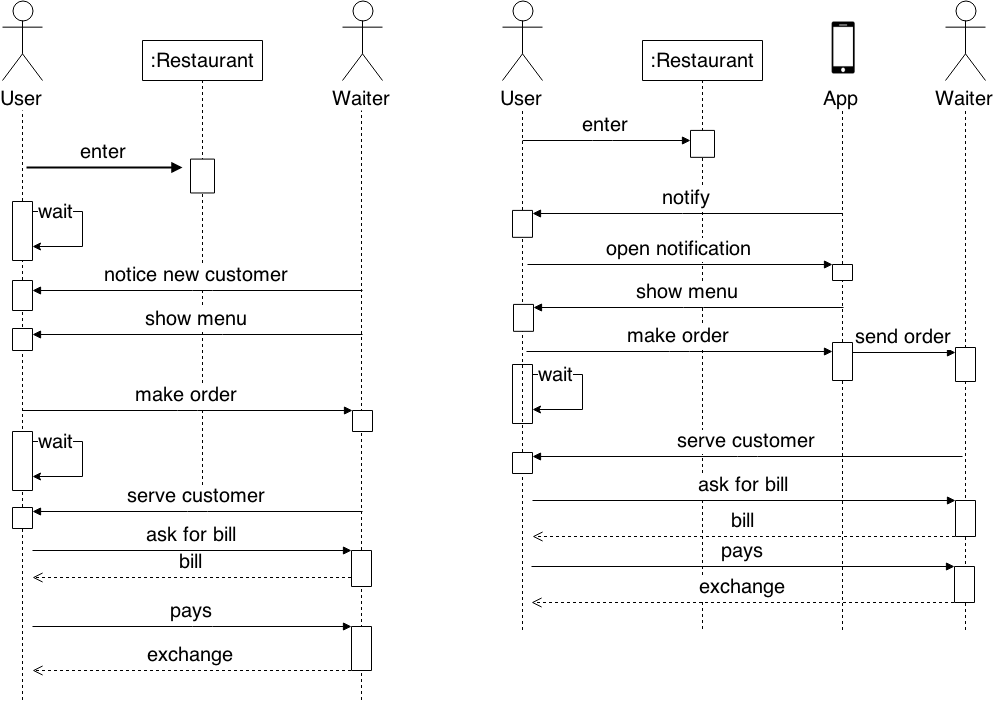
\includegraphics[width=1\textwidth]{figures/smart-restaurant}
    \caption{Sequence diagram showing the interactions between
    the customer and the waiter in a normal restaurant (on the left)
    and in a Smart Restaurant(on the right)}
    \label{fig:smart_restaurant}
\end{figure}

\subsection{Customers}
\label{sub:customers}
As it is shown in figure~\ref{fig:smart_restaurant} some interactions between
the customer and the waiter can be replaced by a mobile app.
For this group of users, the main feature is to allow them to place
the orders using their smartphones. The mobile app detects in which table
the customer is in and sends that information to the web application that the
Owners use. When the customer places his order, he does not need to type
the number of the table. This way, the customer will get his orders
processed faster.

\subsection{Waiters}
\label{sub:waiters}
% Features
This group of users is responsible for processing the customers' orders.
As already mentioned, the smart restaurant solution does not aim to replace
the waiters. It tries to make their job easier. In order to do that,
there is a web application where waiters can check who is requesting them.
Since the mobile app for customers allows them to request a waiter or to place
an order, the web application for waiters allows them to see the customers'
requests. As soon as the customer requests a waiter or place an order,
the web application shows that information and waiters can see from which
table the request is coming from.

\subsection{Owners}
\label{sub:owners}
Before customers and waiters can use this solution, the restaurants' owners
need to do some configurations in order to set everything up.
There is a mobile app for owners that allows them to turn their normal
restaurants in smart ones.
Using this mobile app, owners can configure the menu and the tables.
As already mentioned, this solution uses BLE beacons. To configure
the restaurant's tables, the owners need to perform the following steps:
\begin{itemize}
  \item Deploy one beacon in each table;
  \item Open the mobile app for owners;
  \item Login in the app;
  \item Select the option to configure the tables;
  \item Move the mobile device close to the beacon;
  \item Once the beacon has been detected, select it and type the number
  of the corresponding table
\end{itemize}
Once these steps are done, now they just have to configure the name of the
restaurant and its menu. This menu will be shown to the customers after they
have been notified that they entered in a smart restaurant.

\subsection{Requirements}
\label{sub:requirements}
In order to be able to develop this solution and know, which features are
needed, we need to define the requirements, summarized in table
\ref{table:requirements}. For each requirement, there is an unique
identifier, its description and for which type of user it provides value.
Further, in section \ref{sec:preliminary_results} we will check which
requirements are met by this solution.
% Please add the following required packages to your document preamble:
% \usepackage{graphicx}
\begin{table}[h]
\centering
\resizebox{\textwidth}{!}{%
\begin{tabular}{|l|l|l|}
\hline
{\bf ID} & {\bf Requirement}                                                                                            & {\bf Type of user} \\ \hline
R1       & \begin{tabular}[c]{@{}l@{}}Customers must be allowed to place their \\ orders with a mobile app\end{tabular} & Customers          \\ \hline
R2       & When customers place an order, they must not need to write the table's number                                & Customers          \\ \hline
R3       & Customers must be allowed to request a waiter using a mobile app                                             & Customers          \\ \hline
R4       & Waiters must be able to see the orders that come from the customers' mobile app                              & Waiters            \\ \hline
R5       & Waiters must be able to see from which table an order comes from                                             & Waiters            \\ \hline
R6       & Waiters must be able to see when a customer requests a waiter                                                & Waiter             \\ \hline
R7       & Owners must be able to configure the restaurant's name and menu using a mobile app                           & Owners             \\ \hline
R8       & Owners must be allowed to configure the mapping between the tables and beacons using a mobile app            & Owners             \\ \hline
\end{tabular}
}
\caption{Requirements table}
\label{table:requirements}
\end{table}


%!TEX root = ../paper.tex

\section{Solution Architecture}
\label{sec:solution_architecture}
% Main components: Mobile apps, web app, BaaS, Beacons
After explained how is the experience of the Smart Restaurant for waiters,
customers and owners, the main components of the solution will be described,
the technologies that were used and how they interact with each other.
Figure~\ref{fig:architecture_base} shows the main components that were
implemented in order to be able to offer the Smart Restaurant experience,
described in section \ref{sec:smart_restaurant_experience}.
Also, for each component we point out the type of user that will interact
with it.
As the figure shows, the main components are the following:
\begin{description}
  \item[ibeacons]: The BLE beacons that use the ibeacon protocol explained
  in section \ref{sec:introduction}
  \item[Backend]: Which will store persistent data about the restaurants,
  such as, the restaurants' menus, the orders, and the mapping between
  the tables and the beacons' identifiers
  \item[Smartphone] Where will run the mobile apps, for the customers
  and for owners (described in section \ref{sec:smart_restaurant_experience})
  \item[Web application]: The waiters will use this to check the
  customers' orders.
\end{description}

\begin{figure}[!ht]
  \centering
    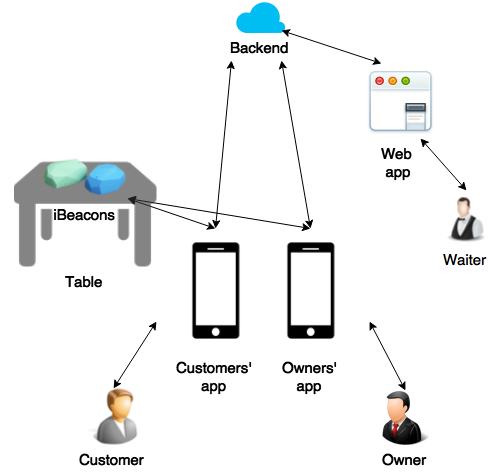
\includegraphics[width=0.7\textwidth]{figures/architecture_base}
    \caption{Main components of Smart Restaurant solution}
    \label{fig:architecture_base}
\end{figure}

\subsection{Backend}
\label{sub:backend}
The backend is the component that supports the mobile and web applications
that are used by the three main groups of users. It stores the data that is
needed for the other applications. This component was not implemented from
scratch, because we only need to be able to store persistent data and to
retrieve it. Instead of writing all the code to create the backend, we
are using a Backend as a Service (BaaS), which is Parse\footnote{http://parse.com}
\cite{parse}.
We only needed to create the collections and their structure.
It offers a REST API\cite{restful} that allow to perform the
Create Read Update and Delete (CRUD) operations
on the collections.
It also offers Software Development Kits (SDKs) for many platforms.
In our implementation we used the
Android\footnote{http://www.android.com} and
Javascript\footnote{http://developer.mozilla.org/en-US/docs/Web/JavaScript/About\_JavaScript}
SDKs. The Android SDK was used in the mobile apps (see \ref{sub:mobile_apps})
and the Javascript SDK was used in the web application
(see \ref{sub:web_app_for_waiters}).

\subsection{Mobile Apps}
\label{sub:mobile_apps}
% Two mobile apps
% (owners and customers)
% Technologies: App Android, BaaS Parse.com
% Package diagram
% Layer diagram for lib
As it is mentioned in section \ref{sec:smart_restaurant_experience}, our
solution for Smart Restaurants has two mobile apps. One for customers and
another one for Owners. Both are Android applications. Both apps are
part of the same project. The project is organized according to the
package diagram in figure~\ref{fig:package_diagram_android}, that shows
that the Android project is composed by three modules:
\begin{description}
  \item[lib]: Library that offers an API to scan for nearby beacons and
  to fetch data from and to the backend. This library uses the Parse Android
  SDK.
  \item[ownersapp]: Android app for restaurants' owners. This app uses
  the lib module to be able to scan for beacons and to get the relevant
  data from the backend
  \item[clientapp]: Android app for customers. This app also uses the lib
  module.
\end{description}

\begin{figure}[!ht]
  \centering
    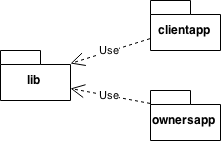
\includegraphics[width=0.4\textwidth]{figures/package_diagram_android}
    \caption{Package diagram of the Android project}
    \label{fig:package_diagram_android}
\end{figure}

The ownersapp and clientapp use the lib module to handle the beacons and
the communication with the backend. They only implement the user interface
and use the lib. Figure~\ref{fig:android-uml} shows the main classes
that implement the lib's logic that are the following:
\begin{description}
  \item[BeaconsManager]: Handles the beacons and offers methods to
  start scanning and stop the current scan process.
  \item[DataStore]: This class implements methods to fetch data from and to
  the backend, for instance, to login the user. These methods receive a callback
  that handles the result because the requests to the backend are asynchronous,
  which means that the user interface does not block waiting for the
  response.
  \item[DataStoreCallback]: This is used by most of the methods in DataStore
  class. This offers an interface that each specific backend's response
  handling should implement.
  \item[DataStoreObject]: Since we have speficied, in the backend, which
  collections we have and their structure, we have classes, that inherit from
  this one, that are wrappers for the raw data that comes from the backend.
\end{description}

\begin{figure}[!ht]
  \centering
    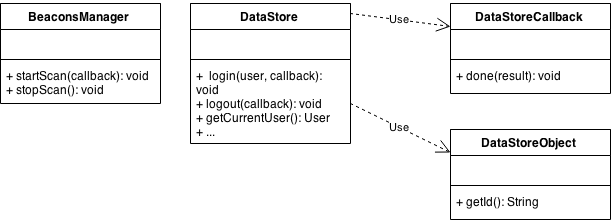
\includegraphics[width=0.8\textwidth]{figures/android-uml}
    \caption{Main classes of the lib module}
    \label{fig:android-uml}
\end{figure}

\subsection{Web App for Waiters}
\label{sub:web_app_for_waiters}
% Web app for waiters
% Technologies used: meteor, BaaS
% meteor: web sockets, live
As mentioned before, there is a web application for waiters. They can
check the coming orders.
This application was implemented using the
Meteor\footnote{http://www.meteor.com}\cite{meteor} framework which allows developers
to write web applications using Javascript in both client and server side.
Using this framework we can set up a new application issuing a single command.
It uses websockets\cite{websockets} to offer reactivity, which means,
when the data changes on the server,
the client will be automatically updated, so the users do not need to
refresh the web page in order to see the updates. We chose to use this
because it allows rapid prototyping and the reactivity feature is important
because, this waiters, only need to look at the screen to know which
orders they have to process next.

%!TEX root = ../paper.tex

\section{Conclusion and Future Work}
\label{sec:conclusion_and_future_work}
We have seen that BLE beacons can be used to develop proximity-based
mobile applications. This paper showed that we can use this technology
to create a new experience inside restaurants.
First, we saw some examples of applications using beacons and software
for restaurants. Some ideas were extracted in order to combine them.
On one side, how to use the beacons and on the other side, which
features are most used in a software solution for restaurants.
Our solution aims to reach customers, waiters and owners.
Customers can use a mobile app to place their orders.
Owners also have a mobile app to manage the restaurant's menu and to
configure the mapping between the beacons and the tables.
This mapping is what allows waiters to know which table a given order
comes from
and customers to not have to type the number of the table.
This solution also offers, to waiters, a web application were they
can see the orders.
We have established some requirements, which are the main
features that we aim to provide.
Our smart restaurant solution implements, aproximately,
88\% of all requirements. The only feature it does not offer is
the payment using the mobile app.

In the future, we are going to try to integrate our
prototype with an existing solution in order to avoid
restaurants' owners having to provide the same information
to two different applications. During the development
of this prototype we faced some challenges, such as
getting the beacons' signals and extract some useful
information from that. From these challenges, we
realized that developing proximity-based mobile
apps using this technology can become an hard task
because, we need not only to implement the mobile app
but also a backend where we map the beacons to
useful information that apps can use. Also, the users
need to download a new app for each proximity-based
service they want to use. We want to change this
by creating a framework to develop such services
in such a way that the user only needs one app
to discover them and use them and developers
can develop their proximity-based services
without the need of implementing a backend
themselves.

\appendix
%!TEX root = ../paper.tex

\section{Appendix} % (fold)
\label{sec:appendix}


% -------------------------------------
% Bibliography
% -------------------------------------
\bibliographystyle{ieeetr}

\bibliography{references.bib}

\end{document}
